% !TeX root = ../Thesis.tex

%************************************************
\chapter{Introduction}\label{ch:introduction}
%************************************************
\glsresetall % Resets all acronyms to not used

Start a chapter with text and not with a section header.
Open the \emph{ClassicThesisConfig.tex} file and fill in the required information.

\section{First Section}
\label{sec:firstsection}

After a section there should always be text before the next section.
The first paragraph is always without indentation.
Starting from the second paragraph, there is an indentation.

Here is an equation without numbers for referencing:
\begin{align*}
	\underbrace{
		\begin{pmatrix}
			\mathcal{B}_1 \\
			\mathcal{B}_2 \\
			\vdots        \\
			\mathcal{B}_R
		\end{pmatrix}
	}_{\mathcal{B}}
	= \underbrace{
		\begin{pmatrix}
			H_{1,1} & H_{1,2} & \hdots & H_{1,T} \\
			H_{2,1} & H_{2,2} & \hdots & H_{2,T} \\
			\vdots  & \vdots  & \ddots & \vdots  \\
			H_{R,1} & H_{R,2} & \hdots & H_{R,T}
		\end{pmatrix}
	}_{H_{A\rightarrow B}}
	\cdot  \underbrace{
		\begin{pmatrix}
			\mathcal{A}_1 \\
			\mathcal{A}_2 \\
			\vdots        \\
			\mathcal{A}_T
		\end{pmatrix}}_{\mathcal{A}}
\end{align*}

Here is an equation that you can reference:
\begin{align}
	\underbrace{
		\begin{pmatrix}
			\mathcal{B}_1 \\
			\mathcal{B}_2 \\
			\vdots        \\
			\mathcal{B}_R
		\end{pmatrix}
	}_{\mathcal{B}}
	= \underbrace{
		\begin{pmatrix}
			H_{1,1} & H_{1,2} & \hdots & H_{1,T} \\
			H_{2,1} & H_{2,2} & \hdots & H_{2,T} \\
			\vdots  & \vdots  & \ddots & \vdots  \\
			H_{R,1} & H_{R,2} & \hdots & H_{R,T}
		\end{pmatrix}
	}_{H_{A\rightarrow B}}
	\cdot \underbrace{
		\begin{pmatrix}
			\mathcal{A}_1 \\
			\mathcal{A}_2 \\
			\vdots        \\
			\mathcal{A}_T
		\end{pmatrix}
	}_{\mathcal{A}}
	\label{eqn:example}
\end{align}

\subsection{Referencing}

Take a look in the following list to reference sections, figures and equations:
\begin{itemize}
  \item \Cref{sec:firstsection}
  \item \Cref{fig:channel}
  \item \Cref{eqn:example}
\end{itemize}

Don't forget to cite all your sources properly, e.g. \cite{1975:Wyner}.

\subsection{Acronyms}
For acronyms you should use the \emph{glossaries} package and put your acronyms
in the \emph{Acronyms.tex} file. The first acronym is always
written in it's long form, the following occurrences are abbreviated: first
occurrence \gls{SNR}, second occurrence \gls{SNR}, plural \glspl{SNR}.

\subsection{Examples on Figures}

\sloppy
When using figures:
\begin{itemize}
	\item Prefer vector graphics whenever possible. See \cref{fig:channel,fig:example}
		for examples to create them directly from \LaTeX code.
	\item You might find the \href{https://github.com/matlab2tikz/matlab2tikz}{matlab2tikz}
		library useful. There are also many python libraries to create tikz images.
	\item When using TikZ, it takes time and memory to recompile graphics. Pdflatex
		caches generated figures when invoked with the \lstinline|--enable-write18| switch.
		Graphics are then only recompiled if you uncomment/use the command
	\lstinline|\tikzset{external/remake next}| within a figure environment.
	\item Figures should always appear after the first reference, either in the text
		or at the top of the same page as the reference.
	\item Prefer placing figures on separate pages
\end{itemize}


\begin{figure}
	\centering
	% NOTE: You can also include tikz images inline instead.
	\begin{tikzpicture}[
	node distance = 7mm and 18mm,
	  start chain = going right,
	   box/.style = {draw, thick,
	                 minimum height=9mm, minimum width =18mm,
	                 on chain},
	every edge/.style = {draw, -Straight Barb, semithick},
	every node/.style = {align=center},
]

	% Draw boxes for Encoder, Channel and Decoder
	\coordinate[on chain] (in);
	\node (n1) [box]    {Encoder};
	\node (n2) [box]    {Channel};
	\node (n3) [box]    {Decoder};
	\coordinate[on chain] (out);

	% Draw labeled arrow between the boxes
	\draw[->] (in) -- node[above] {Message \\ $\mathcal{K}$} (n1);
	\draw[->] (n1) -- node[above] {Codeword\\ $X_{\mathcal{K}}$} (n2);
	\draw[->] (n2) -- node[above] {Output  \\ $Y$} (n3);
	\draw[->] (n3) -- node[above] {Estimate\\ $\widehat{\mathcal{K}}$} (out);
\end{tikzpicture}
	\caption[Communication Channel]{A channel model}
	\label{fig:channel}
\end{figure}

\subsection{Examples on Tables}

You can find an example table in \cref{tab:disasters} using the \emph{tabular} environment.
Note the use of horizontal lines from the \emph{booktabs} package
(\lstinline|\toprule|, \lstinline|\midrule|, and \lstinline|\bottomrule|) and removed
whitespace at both sides of the table (\lstinline|@{}|) as proposed by Markus
Püschel.\footnote{\url{https://www.inf.ethz.ch/personal/markusp/teaching/guides/guide-tables.pdf}}

\begin{table}
	\centering
	\begin{tabular}{@{} lclr @{}} % @{} removes white spaces
		\toprule
		\tableheadline{Disaster} & \tableheadline{Year} & \tableheadline{Country} & \tableheadline{Area (km\textsuperscript{2})} \\
		\midrule
		Nepal earthquake        & 2015 & Nepal             & 3\,610      \\
		Cyclone Pam             & 2015 & Vanuatu           & 12\,190     \\
		Ludian earthquake       & 2014 & China             & 1\,487      \\
		Typhoon Haiyan          & 2013 & Philippines       & 71\,503     \\
		Christchurch earthquake & 2011 & New Zealand       & 1\,426      \\
		East Africa drought     & 2011 & East Africa       & 2\,346\,466 \\
		Tropical storm Washi    & 2011 & Philippines       & 104\,530    \\
		Tohoku earthquake       & 2011 & Japan             & 83\,955     \\
		Haiti earthquake        & 2010 & Haiti             & 27\,750     \\
		Afghanistan blizzard    & 2008 & Afghanistan       & 652\,864    \\
		Sichuan earthquake      & 2008 & China             & 485\,000    \\
		Cyclone Nargis          & 2008 & Myanmar           & 676\,578    \\
		\bottomrule
	\end{tabular}
	% Use alternative short title for table of contents
	\caption[Large-scale natural disasters]{Large-scale natural disasters in the last ten years}
	\label{tab:disasters}
\end{table}

\section{Margin Notes}

Especially in the standard SEEMOO template with wide margins, you are
\marginpar{Here you can add text to the margin. For example, to
summarize the section next to it.} encouraged to insert text into the
margins. If you decide to do so, plan to have at least one margin note
per double page.

\section{Some Example Text}
\lipsum[3]


\begin{figure}
\begin{wide}
	\captionsetup{width=\linewidth}
	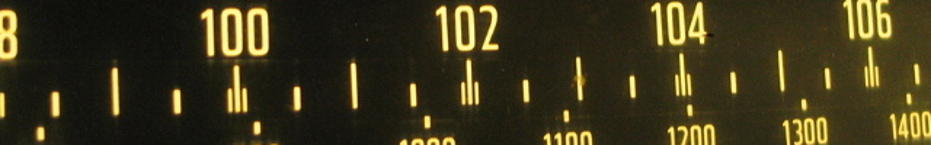
\includegraphics[width=\linewidth]{seemoo-header.jpg}
	\caption{Test of the \lstinline|wide| environment. Make sure to set the width of the figure/table to \lstinline|linewidth|. The environment is useful for more complex and especially full-page figures.}
	\label{fig:wideexample}
\end{wide}
\end{figure}
